\documentclass[conference]{IEEEtran}
\IEEEoverridecommandlockouts
% The preceding line is only needed to identify funding in the first footnote. If that is unneeded, please comment it out.
\usepackage{cite}
\usepackage{amsmath,amssymb,amsfonts}
\usepackage{cite}
\usepackage{algpseudocode}
\usepackage{graphicx}
\usepackage{textcomp}
\usepackage{xcolor}
\usepackage{amsthm}
\usepackage{algorithm}
%\usepackage{algorithmic}
\usepackage{epstopdf}
\usepackage{subfigure}
\usepackage{verbatim}
\usepackage{diagbox}



\newcommand{\tabincell}[2]{\begin{tabular}{@{}#1@{}}#2\end{tabular}}
\def\BibTeX{{\rm B\kern-.05em{\sc i\kern-.025em b}\kern-.08em
    T\kern-.1667em\lower.7ex\hbox{E}\kern-.125emX}}
\begin{document}

\title{Workload-Aware Scheduling for Heterogeneous-Storage Data Analytics\\
}

\author{\IEEEauthorblockN{name1, name2, name3, and name4}
\IEEEauthorblockA{State Key Lab. for Novel Software Technology, Nanjing University, CN\\
Email: email address, \{email address\}@nju.edu.cn}}


\maketitle
%Since the read speeds of diverse storage devices are quite different, the unbalanced use on either specific type of storage or particular device would easily overload them, making them being hotspots and finally worsen the read performance for analytical tasks.
\begin{abstract}
A trend in nowadays data centers is that equipped with SSD, HDD, etc., heterogeneous storage devices are widely deployed to meet different demands of various big data workloads. Since the read speeds of diverse storage devices are quite different, the unbalanced use on either specific type of storage or particular device easily elongates the latency on reading data, worsening the overall performance for analytical tasks. In this paper, we formulate Workload-Aware Scheduling problem for Heterogeneous storage devices (WASH). To solve this proposed problem, we design a randomized algorithm (WASH-rdm) which chooses source devices based on delicate calculated probabilities and can be proved concentrated on its optimum with high probability through our theoretical analysis. Extensive experiments show that WASH-rdm reduces the reading time for tasks by up to 55\% over the state-of-the-art baseline algorithm.
%as well as show its NP-hardness

\end{abstract}

\begin{IEEEkeywords}
big data analytics, heterogeneous storage devices, workload-aware scheduling
\end{IEEEkeywords}

\section{Introduction}

Nowadays, there are new trend that data centers have a variety of data analytical workloads, e.g., some data streaming applications like Storm
\cite{b40}, and other machine learning based applications like Grep \cite{b27}. The different workloads might have different requirements on storage performance \cite{b28} \cite{b29} \cite{b30} \cite{b31}. For example, Storm is a compute-intensive application whose computation relies significantly on the I/O performance while Grep is an I/O-intensive application which has high throughput on data processing. In order to meet these demands, a lot of heterogeneous storage devices \cite{b6} have been widely deployed in big data analytics frameworks, e.g., Hadoop \cite{b14} and Spark\cite{b15}.

However, the heterogeneity of these devices would easily lead to the divergent read performance due to two main aspects. First, the different types of storage, e.g. SSD \cite{b32} and HDD \cite{b33}, naturally results in different read performance. As shown in Fig.~\ref{Fig:motivation} reading the same amount of data from HDD takes almost twice longer than that from SSD. Second, the number of data fetching concurrently also affects read performance. As further shown in Fig.~\ref{Fig:motivation}, when the number of data fetching increases, the reading time also increases as a result of parallel use.%when the number of tasks increases, the reading time for each task will also increase.
%when there are a large number of tasks reading data concurrently from specific device, read performance is also affected

% unbalanced usage on storage device
Due to the different read performance, traditional scheduling may result in relatively longer task reading time. More specifically, when tasks fetch data from those disks with high-performance, they often spend less time on I/O, compared with those low-performance disk. Furthermore, the I/O queries containing too many data analytical tasks may easily overload the storage devices. As a result, disks with poor read performance or heavy workload directly elongates the I/O performance of analytical tasks.

\begin{figure}[!t]
	\centering
	\includegraphics[height=1.8in]{fig_motivation5.eps}
	\caption{Comparisons of (1) reading time for one piece of data with unified size (64MB) on various storage, i.e., SSD and HDD. (2) reading time for various I/O workloads, i.e., concurrently data fetching.}
	\label{Fig:motivation}

	\vspace{-0.4cm}
\end{figure} 

%However, due to the divergent read performance of different storage and the cumulative workload of the storage, its hard to hard to achieve this aim. 
 
Thus, we propose to focus on dealing with unbalanced use on heterogeneous storage devices in this paper. However, due to the multiple replicas of data, how to choose these feasible locations is also a big challenge.
Most of the previous researches have already focused on heterogeneous computing resources \cite{b25}\cite{b26}\cite{b35}\cite{b36}, but ignore the heterogeneous storage devices. Although some works have also already considered heterogeneous storage devices \cite{b6}\cite{b7}, I/O workloads and multiple data replicas are not considered. In contrast, we formulate the Workload-Aware Scheduling problem for Heterogeneous storage devices as well as show its NP-hardness. Afterwards, we propose a randomized algorithm (WASH-rdm) with guaranteed performance by carefully choosing source device based on delicate calculated probabilities.
%We focus on two aspects. One is the read performance of the disk itself, the other is the load of the disk, that is, the number of tasks that are reading the data from the disk. Focus on the above two points, we formulate it as an optimization problem and propose a heuristic algorithm (WASH-greedy) and a random algorithm (WASH-rdm) with guaranteed performance to solve the problem. %Experiments show that the performance of the proposed algorithm is 55\% better than the Storage-unaware scheduling mechanism. 
More concretely, our contributions are as follows: 

\begin{itemize}
%\item We present the necessity of sloving this problem by showing impact of reading data phase during the task execution.
\item To balance the I/O workloads on heterogeneous storage devices, we propose Workload-Aware Scheduling problem for Heterogeneous storage devices(WASH) which is shown as a NP-hard problem. 
\item We propose randomized algorithm with guaranteed-performance. WASH-rdm can be proved concentrated around its optimum with high probability, i.e., 1 - O($e^{-t^2}$), where $t$ is the concentration bound.
\item The results of our extensive simulations show that our proposed WASH-rdm improves by up to 55\% over the art-of-the-state algorithm in terms of average tasks reading time.
%compared with the storage-unaware scheduling mechanism and by 20\% 
\end{itemize}

The rest of the paper is organized as follows. In Section \ref{RELATED_WORKS}, we present the related works of the WASH problem. 
Then our system model and our algorithm are proposed in Section \ref{SYSTEM_MODEL} and Section \ref{DESIGN_ALGORITHM}, respectively. 
In Section \ref{Analysis}, theoretical analysis of our proposed WASH-rdm is presented.
At last, we conclude this paper in Section \ref{CONCLUSION} by summarizing our main contributions.


\section{RELATED WORKS}\label{RELATED_WORKS}
The related works consist of two main parts. For the first part, due to limited bandwidth, some works focus on data locality to reduce the execution delay of data analytics. However, in heterogeneous scenario, it is not enough to consider data locality alone. Thus, some other studies have been carried out to accelerate data analytical tasks by considering hardware heterogeneity \cite{b1} \cite{b6} \cite{b19} \cite{b8}.

\textbf{Fetching Data locally.} Due to the limited network bandwidth in data center, a large amount of data transmitted between nodes before task execution, will greatly affect the performance of data analytics. Therefore, processing data locally as much as possible actually improves the performance, e.g., deploying tasks to the nodes where the input data is stored. 
%delay when the job that should be scheduled next according to fairness cannot launch a local task, it waits for a small amount of time, letting other jobs launch tasks instead
In order to improve data locality, Matei \cite{b2} proposed delay scheduling, which keeps jobs waiting for a while until queuing delay reaches to a presetted threshold or there is idle resource at local.
%a little time instead of launching local tasks when local resources are scarce. %can't launch a local task. Delay scheduling considers that when a node has idle slots, priority should be given to  the tasks whose input data is stored at that node, and delay to schedule tasks whose related data is not stored at that nodes. 
Ganesh \cite{b3} made multiple replicas for high-frequency data by analyzing the number of their accesses, improving the data locality. 
Cristina \cite{b4} proposed a distributed adaptive data replication algorithm DARE, which helped the scheduler for better data locality. 
Jalaparti \cite{b5} believed that most of the production work is repetitive and predictable, by which the scheduler could make scheduling plan ahead. 
%Coordinating the tasks and data placement of these jobs can effectively reduce bandwidth usage, further, improving data locality. 
All of these works improves the performance of data analytics by considering data locality. 
However, due to the fact that local disks might have high I/O workloads, previous strategies would elongate the latency of local tasks.

\textbf{Fetching Data Remotely.} 
In heterogeneous cluster, data fetching remotely from those devices with higher performance on I/O could be better than that from local ones.
%since tasks fetching data from high-performance disks of other nodes might have low reading time, considering data locality alone is not enough to speed up analytical tasks. 
However, most of the researches only focused on heterogeneous computing resources \cite{b25} \cite{b26} \cite{b35} \cite{b36} \cite{b6}, but ignored the heterogeneous-storage devices. For example, Xu \cite{b6} considered the current usability of underlying hardware (CPU, memory, I/O), but didn't consider the performance on different storage hardware. 
In Hadoop 2.3, HDFS\cite{b19} took the heterogeneous storage feature into consideration, which supported six storage strategies. Users could choose one of these strategies to store files according to their demands.
%is proposed considers heterogeneous storage devices and supports multiple storage strategies. One of the storage strategies is named , that is, one replicas is stored in SSD, and the rest is stored in HDD. 
%However, the task scheduling strategy is not aware of the disk's performance.
Based on such feature, Pan \cite{b7} proposed H-Scheduler to launch tasks according to the different performance between HDD and SSD. However, such scheduling mechanism used heuristic method to read data from HDD or SSD, ignoring unbalanced use among disks.
%However, with the increasing trend of heterogeneous storage devices, it is one-sided to divide the storage devices into two categories. 
Wang B \cite{b8} used Markov to model the use of nodes in the cluster to deploy data reasonably, but ignored tasks reading time. %However, the scheduling problem of reading tasks is not considered, and the heterogeneity of different storage media is not considered, either. %These works do not accurately define the differences between storage hardwares, and there is still a situation where a large number of tasks read data from low-speed devices, causing bottlenecks.
%in a blind way

Among these works, either the reading time of the tasks or the target disks is not considered. Thus, there is still a situation where a large number of tasks overload storage devices, causing bottlenecks.
The difference between those works and ours is that our work specifically models the reading differences and the I/O workloads among disks. Then, each task chooses source disks based on delicate calculated probabilities, to speed up its reading time.

\section{SYSTEM MODEL AND PROBLEM FORMULATION}\label{SYSTEM_MODEL}
In this section, we first introduce the background of heterogeneous storage devices used in data analytics and then build the system model. After that, we formulate the Workload-Aware Scheduling problem and show its NP-hardness. 

\subsection{Background and motivation}\label{AA}

In data center, Hadoop and Spark widely use heterogeneous storage devices to support different workloads. For example, in MapReduce framework, Shuffle stage \cite{b42} \cite{b41} usually has a large requirement on I/O for storing intermediate data. In order to meet this demand, Crail \cite{b37} is proposed to be a high-performance I/O architecture for data processing, using NVMe SSD as a supplementary to speed up the Shuffle phase.
%with the number of heterogeneous disks increasing, traditional scheduling may lead to disk bottleneck. Before analysing the problem, we will introduce data and replicas as well as job and tasks first.

\textbf{Data and replicas.} In data analytics system, large volume of data is generated, such as GPS information\cite{b38}, system logs\cite{b39}, etc. Due to their massive sizes, a large file is often divided into multiple fixed-size pieces, i.e., one $data$ block, stored in a distributed file system such as HDFS\cite{b19}, whose uniform size is often 64MB or 128MB. However, the disk is usually unreliability, e.g., about 5 to 6 disks are damaged per day in a cluster of 5,000 machines \cite{b32}. In order to avoid such data loss, traditional approach is to keep multiple $replicas$ of each data in storage, e.g., three backups across two racks. Then, one piece of data will be stored in multiple disks with various I/O performance.
% The tasks will be scheduled to node to execute. ,

\textbf{Job and tasks.} A data analytics workload, named a $job$, includes many parallel $tasks$. Since each task must read its related input data before execution from the corresponding disk, the scheduler in data analytics system needs to decide the fetching source for each task among multiple replicas. Note that the completion of a job depends on the straggler tasks.


However, traditional schedulers for data analytics are usually unaware of disks' types and I/O workloads, which often leads to straggler tasks. In contrast, our scheduler is then designed to avoid the stragglers by balancing I/O workloads among heterogeneous storage devices.

\textbf{Motivation and example.}
%In order to improve the performance of data analytics tasks, tasks should read data from high performance and low load disks. 
We will use a simple example to illustrate the importance on choosing heterogeneous storage devices. As shown in Fig.~\ref{Fig:example}, there are two types of disks, i.e., SSD and HDD. The reading time for a data replica from SSD and HDD is $T_1$ = 0.2 and $T_2$ = 0.4, respectively. 
\begin{itemize}
	\item The traditional scheduler deploys tasks like scheduling \uppercase\expandafter{\romannumeral1} of Fig.~\ref{Fig:example}(a), whose reading time for a data replica is $0.4s$ while the reading time of the delicate method, i.e., scheduling \uppercase\expandafter{\romannumeral2}, is $0.2s$. Obviously, the task that reads data from SSD has a shorter reading time than that from HDD, i.e., scheduling \uppercase\expandafter{\romannumeral2} is better than scheduling \uppercase\expandafter{\romannumeral1}.

	\item In Fig.~\ref{Fig:example}(b), since the number of fetching data concurrently is 3 from SSD, the reading time of scheduling \uppercase\expandafter{\romannumeral1} is then $0.2s * 3 = 0.6s$, while the task reading time of the delicate method, i.e., scheduling \uppercase\expandafter{\romannumeral2}, is $max\{0.2s * 2, 0.4s\} = 0.4s$. Apparently, the tasks that read data from storage device with a lower I/O workloads have a shorter reading time than that from higher ones, i.e., scheduling \uppercase\expandafter{\romannumeral2} is better than scheduling \uppercase\expandafter{\romannumeral1}.
\end{itemize}

This simple case reveals two important findings: (1) the types of heterogeneous storage devices affect task reading time. (2) the I/O workloads of storage devices also have effects on task reading time. In order to shorten the task reading time, we should take both of the these two findings into consideration.

%\begin{figure}[!t]
%\begin{minipage}[!t]{0.51\textwidth}
%	\centering
%	\subfigure[Type of storage. Scheduling 1 = $0.4s$, Scheduling 2 = $0.2s$]{\label{Fig:example1}\includegraphics[height=1.1in]{fig_example1_3.eps}}	
%	\subfigure[Load of storage.  Scheduling 1 = $0.2s*3$, Scheduling 2 = $max\{0.2s*2, 0.4s*1\}$]{\label{Fig:example2}
%	\includegraphics[height=1.1in]{fig_example2_2.eps}}
%	\caption{Two aspects that affect the task reading time: (1) type of storage, \protect\\(2) Load of storage. Delicate method, i.e., Scheduling 2, improves 50\%, 33\% over scheduling 1, respectively.}
%	\label{Fig:example}
%\end{minipage}
%\end{figure}
%width=4.78cm width=3.95cm

\begin{figure}[!t]
\centering
    \begin{minipage}{4.78cm}
        \includegraphics[height = 2.8cm]{fig_example1_5.eps}
        \centerline{\footnotesize{\uppercase\expandafter{\romannumeral1} = $max$\{0, $0.4s$\},\quad}}\\
        \centerline{\footnotesize{\uppercase\expandafter{\romannumeral2} = $max$\{$0.2s$, 0\}.\quad}}\\
         \centerline{(a) Type of storage.}\\
    \end{minipage}
    \begin{minipage}{3.95cm}
        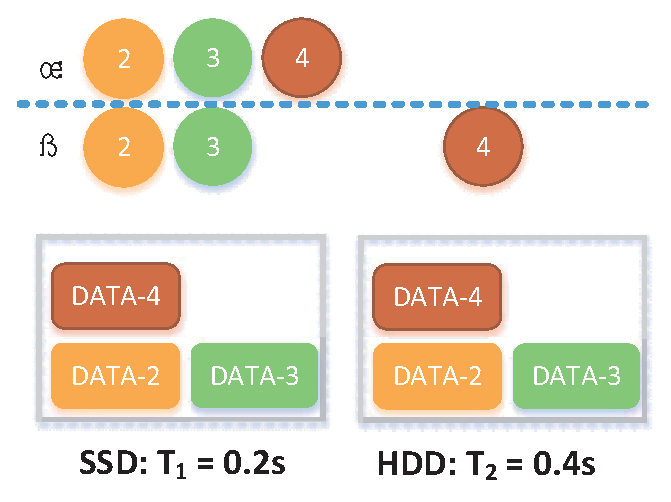
\includegraphics[height = 2.8cm]{fig_example2_4.eps}
        \centerline{\footnotesize{\uppercase\expandafter{\romannumeral1} = $max$\{$0.2s*3$, 0\},\quad}}\\
        \centerline{\footnotesize{\uppercase\expandafter{\romannumeral2} = $max$\{$0.2s*2$, 0.4s\}.}}\\
         \centerline{(b) Load of storage.\quad}\\
    \end{minipage}
    \vspace{-0.4cm}
    \caption{Two aspects that affect the task reading time: (a) Type of storage, (b) Load of storage. Delicate method, i.e., Scheduling \uppercase\expandafter{\romannumeral2}, improves 50\%, 33\% over scheduling \uppercase\expandafter{\romannumeral1}, respectively.}
    \label{Fig:example}
    \vspace{-0.4cm}
\end{figure}

%denoted by \{$r_l^1$, $r_l^2$,... $r_l^{C}$\}
\subsection{System Model}

The major notations used are listed in Table~\ref{table-notations}. The data center is equipped with heterogeneous disks, hence we denote by $\mathcal{D}$ the heterogeneous disks set, i.e., $\mathcal{D}$ = \{1, 2, ...,$|\mathcal{D}|$\}. Each disk-$i$ corresponds to a different reading time for only one replica as its reading performance, represented by $T_i$, $i \in \mathcal{D}$.
$\mathcal{M}$ is defined as the set of all data in data center, $\mathcal{M}$ = \{1, 2, ..., $|\mathcal{M}|$\}. Each data-$l$ has $C$ replicas stored in $C$ different disks whose size is $\tau$, e.g., 64MB. $\pi_l^{i}$ is a binary variable indicating whether data-$l$ is stored in disk-$i$ or not. More concretely, we define $\pi_l^{i}$ as
\begin{equation}
\pi_l^{i} =
\begin{cases}
1, &\text{if disk-$i$ stores a replica of data-$l$,}\\
0, &\text{otherwise,}
\end{cases}\nonumber
\vspace{-0.2cm}
\end{equation}

For each of submitted job, it is often divided into parallel tasks by data analytics framework, denoted by $\mathcal{T}$ = \{1, 2,  ..., $\mathcal{|T|}$ \}. Each task-$j$ corresponds to an input data whose index is defined as $\phi_j$. Since there are $C$ replicas for each data stored in different $C$ disks, task-$j$ can read data-$\phi_j$ among those $C$ disks, whose indexes can be represented as \{$d_{1}^j$, $d_{2}^j$,... $d_{C}^j$\}.


$I_i^j$ is a decision variable, indicating whether task-$j$ chooses the replica stored in disk-$i$ as its input or not. Specifically, we define $\pi_l^{i}$ as
\begin{equation}
I_i^j =
\begin{cases}
1, &\text{\tabincell{l}{if task-$j$ chooses the replica stored in disk-$i$,}}\\
0, &\text{otherwise,}
\end{cases}\nonumber
\end{equation}

Then, we denote by $load_i$ the reading time of all tasks from disk-$i$, i.e., $load_{i}$ = $\sum_{j}I_i^j*T_i$. In order to balance the use on heterogeneous storage devices as well as optimize the reading time of data analytical tasks, our objective is to minimize the maximal $load$ of all disks.

\begin{table}[!t]
	\Large
	\centering
	\footnotesize
	\renewcommand\arraystretch{1.2}
	\caption{MAJOR NOTATIONS USED IN THIS PAPER.}
	\label{table-notations}
	\begin{tabular}{c|l}
		\hline\hline
		Variable & Description\\
		\hline
		$T_{i}$ & \tabincell{l}{The time of reading one replica from disk-$i$ \\for only one task without other concurrent tasks} \\
		\hline
		$\phi_j$ & The index of data that task-$j$ needs, as its input \\
		\hline
		$d_{r}^j$ & \tabincell{l}{The index of disk which stores data-$\phi_j$'s $r$-th replica} \\
		\hline
		$\pi_{l}^{i}$ & \tabincell{l}{A binary variable indicating if data-$l$ are \\stored in disk-$i$ or not} \\
		\hline
		$N_i$ & Number of tasks which reads data from disk-$i$ \\
		\hline
		$\tau$ & Unified size of each data replica in data center \\
		\hline
		$C$ & The number of replicas for each data \\
		\hline\hline
		Decision variable & Description\\
		\hline
		${I}_i^j$ & \tabincell{l}{A binary variable indicating if task-$j$ chooses \\ to read the replica stored in disk-$i$ or not}\\
		\hline	
	\end{tabular}
	\vspace{-0.4cm}
\end{table}

\subsection{Workload-Aware Scheduling problem for Heterogeneous storage devices $(\rm{WASH})$} \label{WASH}
%$\mathcal{AP} \mathbb{AP}$ (~/~)
%A large number of tasks are running in the cluster of data centers.
For parallel tasks, if the scheduler is unaware of the heterogeneity of disks, it would easily lead to the unbalanced use on disks, elongating the latency of analytical tasks. To avoid such bottleneck, we propose Workload-Aware Scheduling problem for Heterogeneous storage devices (WASH) whose goal is to minimize the maximal reading time. Detailed description is as follows:
%Finally, by determining the value of the decision variable $I_i^j$, the appropriate disk is selected for each task to read the corresponding data. Detailed description is as follows:
\begin{align}
Min:&\;\;\;\;\;\max\limits_{i}\{\sum_{j}I_i^j*T_i\}\;\;\;\;\;\;[\rm{WASH}]\nonumber\\
s.t. 
&\;\;\;\;\;\sum_{i}I_i^j = 1,\;\;\forall j,\label{task-cons}\\
&\;\;\;\;\;I_i^j \leq \pi_{\phi_j}^{i},\;\;\forall i,j\label{data-cons},\\
&\;\;\;\;\;I_i^j\in\{0,1\},\;\;\forall i,j.\label{def-cons}
\end{align}

%Constraint (\ref{task-cons}) guarantees that task-$j$ can only fetch data $\phi_j$ from those source disks. Constraint (\ref{data-cons}) guarantees that task-$j$ can only select from those disks containing its input data. If one replica of data $\phi_j$ is stored in disk-$i$, then $\pi_{\phi_j}^{i}$ = 1, otherwise $\pi_{\phi_j}^{i}$ = 0. Constraint 3 denotes the domain of decision variables, which can only be 0 or 1. $I_i^j$ = 1 indicates that task-$j$ selects the replica stored on disk-$i$ as input, while $I_i^j$ = 0 is on the contrary.The key to solve WASH problem is to determine the value of decision variables {$I_i^j$}. 
Constraint (\ref{task-cons}) and Constraint (\ref{data-cons}) guarantee that task-$j$ only fetches data-$\phi_j$ from one of those source disks storing its input. 
%$\phi_j$ represents the index of data that task-$j$ needs, $\phi_j$ $\in$  $\mathcal{M}$.
If one replica of data-$\phi_j$ is stored in disk-$i$, then $\pi_{\phi_j}^{i}$ = 1, otherwise $\pi_{\phi_j}^{i}$ = 0. 
The key to solve WASH problem is to determine the value of those decision variables, i.e., {$I_i^j$}. 

%Next, we show the NP-hardness of this problem. More specifically, WASH problem can be reduced from the integer linear programming (ILP) problem. The ILP problem is NP-hard \cite{b9} in general, so as that WASH problem is then NP-hard. The specific proof is as shown follows.

\emph{\textbf{Theorem 1:}} The WASH problem is NP-hard.

\emph{Proof:} See Appendix.

%Alogoritm1
\begin{algorithm}

	\textbf{Require:} Task-$j$ and its input data-$\phi_j$, $\forall j$.

	\begin{algorithmic}[1]
		
		\State $Result$ $\gets$ \{\}\label{WASH-greedy:init}
		\For{each task-$j$} 
			\State \{$d_{1}^j$, $d_{2}^j$,... $d_{C}^j$\} = $f(\phi_j)$
		
			\leftline{\;\;\;\;\;\;$//$ $f(\phi_j)$ is a set of disks storing data-$\phi_j$.}
	
			\State $d_{min}^j$ $\gets$ $\mathop{\arg\min}\limits_{d \in \{d_{1}^j, d_{2}^j,... d_{C}^j\}}$ $\{T_d\}$
			\State $Result$ $\gets$ $Result$ $\cup$
			\{$< j, d_{min}^j>$\}
		\EndFor
%\left \langle \right \rangle
	\State  Each task-$j$ reads data according to $Result$.
	\end{algorithmic}
	\caption{WASH-greedy}\label{WASH-greedy}
\end{algorithm}

\section{DESIGN of ALGORITHMS FOR WASH PROBLEM}\label{DESIGN_ALGORITHM}

The key to minimize the overall reading time for each task is to find the optimal source disk storing its input among the heterogeneous disks. However, due to the NP-hardness of WASH problem, the optimal solutions can't be obtained within polynomial time, unless NP $=$ P. Since it takes less time to read data from higher performance disks than that from lower ones, we first explore a heuristic algorithm, intuitively, which often chooses these disks with higher-performance on I/O, named WASH-greedy. However, due to its preference on high performance disks, WASH-greedy may often overload high-performance disks, making them being bottlenecks. 
%such algorithm always giving preference to disks with high-performance as input for each task
%However, extensive experiments shows that WASH-greedy has a little improvement over the baseline, i.e., Hadoop-default which is storage-unaware. 
Furthermore, In order to solve WASH effectively as well as to avoid bottlenecks, we design a randomized algorithm (WASH-rdm) which chooses source devices based on delicate calculated probabilities and can be proved concentrated on its optimum with high probability, i.e., 1- O($e^{-t^2}$), through our theoretical analysis.

\subsection{Inspiration}\label{Heuristic}
%we first introduce WASH-greedy which is based on a greedy idea that always selects source disk with minimal reading time, i.e. $T_i$, greedily . 
In this subsection, we first introduce WASH-greedy which selects source disk with minimal reading time, i.e. $T_i$, greedily . Then, we will use a simple example to illustrate the process of WASH-greedy. %To be more specific, WASH-greedy is shown as follows:



Algorithm \ref{WASH-greedy:init} shows the details of WASH-greedy. Line 1 initializes $Result$ = \{\}. Line 2-6 is used to select a source disk for each task-$j$. In line 3, function $f$ is used for task-$j$ to find the indexes of those disks which store the input data of task-$j$, i.e., data-$\phi_j$, represented by \{$d_{1}^j$, $d_{2}^j$,... $d_{C}^j$\}. Next, in line 4, the disk with minimal $T_i$ is selected from those $C$ disks. After $\mathcal{|T|}$ iterations, the selections of source disks for $\mathcal{|T|}$ tasks are completed. Then, each task will read its input data according to $Result$.

% After putting the task-$j$ and disk $d_{j_l}$ into the set $Result$, the algorithm completes one assignment of a task.

%Next, an example is given to illustrate the algorithm. In datacenter, there exits a set of heterogeneous disks $\mathcal{D}$= \{$d_1$, $d_2$, $d_3$, $d_4$\} with $T_i$ $T_1$ = 0.3,  $T_2$ = 0.1,  $T_3$ =0.2 and $T_4$ =0.2, respectively. Data set $\mathbb{M}$ = \{$m_1$, $m_2$, $m_3$, $m_4$\} are stored as Fig.\ref{fig1}. Obviously, each data has two replicas. When query tasks $\mathcal{T}$= \{$t_1$, $t_2$, $t_3$, $t_4$\} ($\phi_j$ = j, 1$\leq$j$ \leq$4) comes, the algorithm WASH-greedy runs as follows: %($\phi_j$ = j (1 $\leq$j$ \leq$ 4, task $t_j$'s input is $m_j$ which equals the DATA-j in Fig.\ref{fig1}))

Next, we use an example to illustrate the process of WAHS-greedy. In data center, there exits four heterogeneous disks, i.e., $\mathcal{D}$= \{1, 2, 3, 4\} with $T_1$ = 0.2,  $T_2$ = 0.25,  $T_3$ =0.4 and $T_4$ =0.6, respectively. Furthermore, five pieces of data are stored as shown in Fig.~\ref{fig1}. When a job with five tasks comes, algorithm WASH-greedy runs as follows: %Obviously, each data has two replicas. When query tasks $\mathcal{T}$= \{1, 2, 3, 4\} ($\phi_j$ = j, 1$\leq$j$ \leq$4) comes, the algorithm WASH-greedy runs as follows: %($\phi_j$ = j (1 $\leq$j$ \leq$ 4, task $t_j$'s input is $m_j$ which equals the DATA-j in Fig.~\ref{fig1}))

Initial: Result = \{\}
\begin{itemize}
	\item \textbf{Round 1}:for task-1:
	 f($\phi_1$) = \{1, 2\} \\
	 $1$ = $\arg\min$\{$T_1$ = 0.2, $T_2$ = 0.25\}\\
	Result = Result $\cup$ $\left \langle 1, 1\right \rangle$ = \{$\left \langle 1, 1\right \rangle$\}
	\item \textbf{Round 2}:for task-2:
	f($\phi_2$) = \{2, 3\}\\
	$2$ = $\arg\min$\{$T_2$ = 0.25, $T_3$ = 0.4\}\\
	Result = Result $\cup$ $\left \langle 2, 2\right \rangle$ = \{$\left \langle 1, 1\right \rangle$, $\left \langle 2, 2\right \rangle$\}
	\item \textbf{Round 3}:for task-3:
	f($\phi_3$) = \{3, 4\}\\
	$3$ = $\arg\min$\{$T_3$ = 0.4, $T_4$ = 0.6\}\\
	Result = Result $\cup$ $\left \langle 3, 3\right \rangle$ = \{$\left \langle 1, 1\right \rangle$, $\left \langle 2, 2\right \rangle$,  $\left \langle 3, 3\right \rangle$\}
	\item \textbf{Round 4}:for task  $4$:
	f($\phi_4$) = \{1, 4\}\\
	$1$ = $\arg\min$\{$T_1$ = 0.2, $T_4$ = 0.6\}\\
	Result = Result $\cup$ $\left \langle 4, 1\right \rangle$ = \{$\left \langle 1, 1\right \rangle$, $\left \langle 2, 2\right \rangle$,  $\left \langle 3, 3\right \rangle$, $\left \langle 4, 1\right \rangle$\}	
	\item \textbf{Round 5}:for task-5:
	f($\phi(5)$) = \{2, 4\}\\
	$2$ = $\arg\min$\{$T_2$ = 0.25, $T_4$ = 0.6\}\\
	Result = Result $\cup$ $\left \langle 5, 2\right \rangle$ = \{$\left \langle 1, 1\right \rangle$, $\left \langle 2, 2\right \rangle$,  $\left \langle 3, 3\right \rangle$, $\left \langle 4, 1\right \rangle$, $\left \langle 5, 2\right \rangle$\}	
	
\end{itemize}
\begin{figure}[!t]
	\centering
	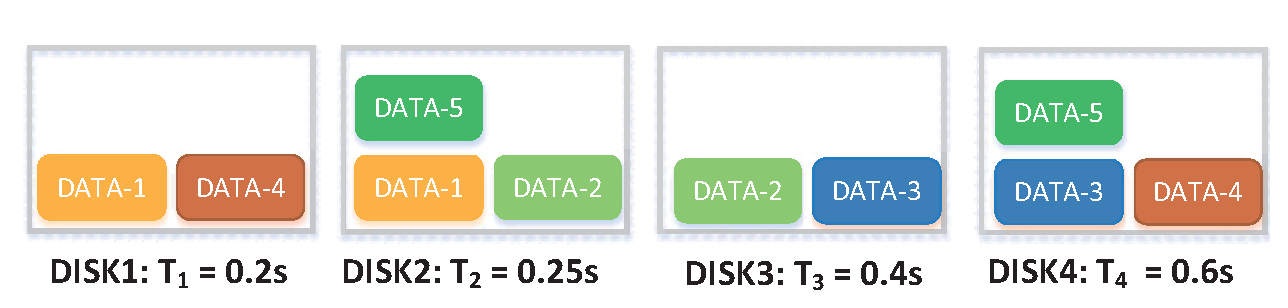
\includegraphics[height=0.8in]{fig1_10.eps}
	\caption{Distribution of five pieces of data across 4 disks.  }
	\label{fig1}
	\vspace{-0.4cm}
\end{figure}
\begin{figure}[!t]
	\centering
	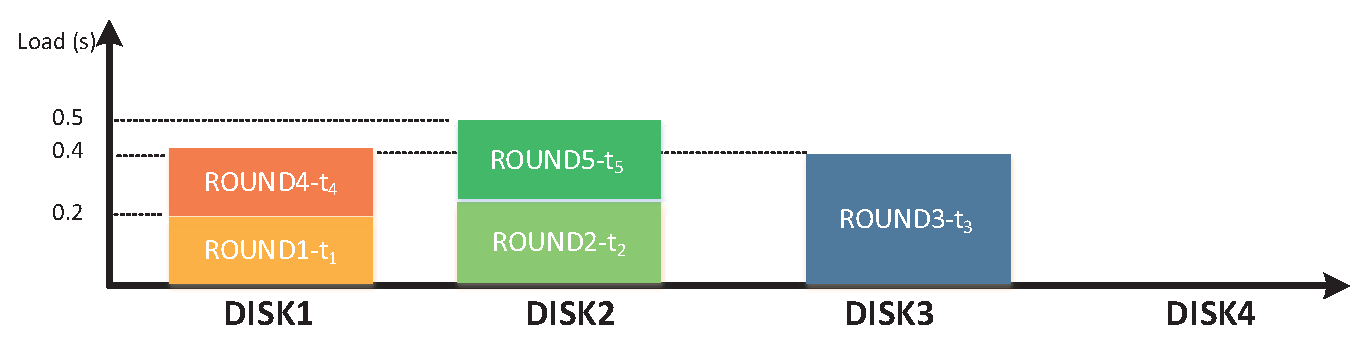
\includegraphics[height=0.8in]{fig2_3.eps}
	\caption{The process of WASH-greedy for the data distributed in Fig.~\ref{fig1}. }
	\label{fig2}
	\vspace{-0.4cm}
\end{figure}

Then, four tasks read data according to the strategy of \{$\left \langle 1, 3\right \rangle$, $\left \langle 2, 1\right \rangle$,  $\left \langle 3, 2\right \rangle$, $\left \langle 4, 1\right \rangle$, $\left \langle 5, 2\right \rangle$, $\left \langle 6, 1\right \rangle$\}.The specific steps of WASH-greedy algorithm is shown in Fig.~\ref{fig2}.

Due to the fact that WASH-greedy always shows its preference on the disks with high-performance for each task, such algorithm may easily overload high-performance disks. Thus, WASH-greedy can't avoid the disks bottleneck, elongating the I/O performance of analytical tasks.

\subsection{Randomized tasks scheduling}\label{Randomized}

%In the previous subsection \ref{Heuristic}, we explore a greedy heuristic algorithm to solve WASH problem, intuitively. 
%However, WASH-greedy could not avoid of the disk bottleneck while a lots of tasks are reading data from a high-performance disk. It is because that WASH-greed always giving preference to disks with high-performance as input for each task. Actually, such scenario are avoided if tasks could be allocated across disks, reasonably. 

In this subsection, we design a randomized algorithm, named WASH-rdm, which avoids disk bottleneck by choosing source devices based on delicate calculated probabilities. Specifically, by relaxing the WASH problem to its relaxation version, i.e., WASH-relaxation, then we use linear programming technique to solve WASH-relaxation. The solution obtained by linear programming technique, in a sense, represents the preference when selecting source disks. Therefore, our WASH-rdm uses such results as a series of probability to choose disk for each task. Subsequently, we prove that WASH-rdm is concentrated on its optimum with high probability, i.e., 1- O($e^{-t^2}$), through our theoretical analysis, where $t$ is the concentration bound.

 \begin{algorithm}
 	%\renewcommand{\thealgorithm}{}
 	\textbf{Require:} Task-$j$ and its input data-$\phi_j$, $\forall j$. %and $d_i$ stores data $\phi_j$.
 	\begin{algorithmic}[1]	
 		\State $Result$ $\gets$ \{\}
 		\State \{$p_i^j$\} = WASH-relaxation		
 		
 		\leftline{\;\;\;\;\;\;$//$ \{$p_i^j$\} is the solution of WASH-relaxation problem. }
 		
 		\State Use \{$p_i^j$\} twice and get $<\{I_i^j\}_1, \{I_i^j\}_2 >$
 		
		\leftline{\;\;\;\;\;\;$//$ Apply rounding strategy twice. }
		\State Select $\{I_i^j\}$ from $<\{I_i^j\}_1, \{I_i^j\}_2>$

		\leftline{\;\;\;\;\;\;$//$ Select $\{I_i^j\}$ which minimizes WASH. }

 		\For{$\forall$ $i$, $j$, ($i \in \mathcal{D}$, $j \in \mathcal{T}$) } 
 			\If{$I_i^j$ == 1}
 			\State $Result$ $\gets$ $Result$ $\cup$ 	
 			\{$\left \langle j, i\right \rangle$\}
 			\EndIf
 		\EndFor	
 		\State Each task-$j$ reads data according to $Result$.
 	\end{algorithmic}
 	\caption{WASH-rdm}\label{WASH-rdm}
 \end{algorithm}

\paragraph{\textbf{Relaxation of WASH}} According to the previous analysis \ref{WASH}, this problem is NP-hard, whose optimal source disk for each task cannot be obtained within polynomial time. But linear programming (LP) problem is solvable within polynomial time as well shows a lower bound for the original problem, a natural point of view is to relax the WASH problem to a LP problem. The method is to change the domain of decision variables from integer domain \{0, 1\} to real one [0, 1], i.e., WASH-relaxation. Such process is named \textbf{Relaxation}. Detailed description is as follows: 
%The solution of WASH-relaxation provides a lower bound for the original WASH problem (WASH is a minimization problem. For the maximization problem is on the contrary).
\vspace{-0.2cm}
 \begin{align}
 Min:&\;\;\;\;\;\max\limits_{i}\{\sum_{j}p_i^j*T_i\}\;\;\;\;\;\;[\rm{WASH-relaxtion}]\nonumber\\
 s.t. 
 &\;\;\;\;\;\sum_{i}p_i^j = 1,\;\;\forall j,\nonumber\\
 &\;\;\;\;\;p_i^j \leq \pi_{\phi_j}^{i},\;\;\forall i,j,\nonumber\\
 &\;\;\;\;\;p_i^j \in[0, 1],\;\;\forall i,j.\nonumber
 \end{align}

Then, we use linear programming technique to solve WASH-relaxation whose solutions are fraction distributed in [0, 1]. In a sense, the fraction solutions represents the preference when choosing the source disk for each task. 
 \paragraph{\textbf{WASH-rdm schema}} 
Thus, our WASH-rdm use these fraction as probability to choose source disk for each disk. In this way, the solution in fractional domain is mapped back to integer domain, which is named \textbf{Rounding}. 
Based on relaxation-rounding strategy, we propose WASH-rdm algorithm. 

The detailed of WASH-rdm is shown in Algorithm \ref{WASH-rdm}. Line 1 initializes the set of $Result$. In line 2, we use linear programming technique to solve WASH-relaxation. For the third line, our proposed WASH-rdm uses rounding strategy to convert fractional solution into integer solution. The specific rounding strategy is shown as follows:
 
The value of \{$p_i^j$\}  shows the correlation between task-$j$ and disk-$i$. Then, we can select a disk-$i$ for each task-$j$ with probability \{$p_i^j$\}. The method is that, $\forall j$, we randomly select a fraction $q_j$ from (0,1]. If $q_j$ $\in$ ($\sum\nolimits_{r = 1}^{k-1} p_{r}^{j}$,  $\sum\nolimits_{r = 1}^{k} p_{r}^{j}$], $2 \leq k \leq \mathcal{D} $, then $I_k^j = 1$, otherwise, $I_k^j$ = 0. This approach ensures only one disk can be selected for each task and $Pr[I_i^j = 1] = p_i^j$.
%Specially, if $q_j \leq p_{1}^{j}$, then $I_1^j = 1$ and $I_k^j$ = 0 ($k \in \mathcal{D} - \{ 1\}$).  For each task $t_j$, the corresponding decision variables are \{$p_0^j$,$p_i^j$, ..., $p_i^j$\}. 

In order to obtain more precise solution, we use rounding strategy twice, i.e., line 3. Then, we choose the one which minimizes the WASH between two choices, i.e., power of two choices \cite{b43}. In line 5-9, the results are stored in $Result$. After that, the tasks read the data according to $Result$. 

\section{Analysis of WASH-rdm Algorithm}\label{Analysis}

In this section, we will show that our WASH-rdm is concentrated on its optimum with high probability, i.e., 1- O($e^{-t^2}$), through our theoretical analysis, where $t$ is the concentration bound. Firstly, we prove that the difference between reading time of disk-$i$ contributed by any task-$j$ and its expectation could be bounded by Martingale \cite{b12}. After that, we use Azuma's Inequality to illustrate the gap between the feasible solution and the optimal solution. In the following, we use $SOL$ to represent the feasible solution solved by WASH-rdm, and $OPT$ to represent the optimal solution of WASH problem.

\vspace{0.2cm}
\emph{\textbf{Theorem 2:}} $Pr[SOL - OPT\leq t] \geq 1 - O(e^{-t^2})$.

\emph{\textbf{Proof:}}

Firstly, the contribution on additional workload of each task-$j$ to disk-$i$'s $load$ is expressed as
\vspace{-0.2cm}
 \begin{align}
&\;\;\;\;\;Z_i^j = I_i^j*T_i.
\end{align}

\vspace{-0.2cm}
From the rounding strategy in Algorithm \ref{WASH-rdm}, we obtain
 \vspace{-0.2cm}
 \begin{align}
&\;\;\;\;\;Pr[I_i^j = 1] = p_i^j. \nonumber
\end{align}
%Therefore

\vspace{-0.2cm}
The expectation of $Z_i^j$ then is represented as
\vspace{-0.2cm}
\begin{align}
E[Z_i^j] &= E[I_i^j]*T_i \nonumber\\
&= (Pr[I_i^j = 1] * 1 +  0)*T_i = p_i^j*T_i.\label{prove:expect}
\end{align}

\vspace{-0.2cm}
The difference between $Z_i^j$ and $E[Z_i^j]$ is defined as
 \vspace{-0.1cm}
\begin{align}
Q_i^j = Z_i^j - E[Z_i^j].\label{prove:diff}
\end{align}

%we denote by $L_i^{\mathcal{|T|}}$ the sum of $Q_i^j$ in disk $i$, i.e., 
\vspace{-0.2cm}
For all tasks, we denote by $L_i^{\mathcal{|T|}}$ the sum of their workload difference in disk $i$, i.e., $Q_i^j$ 
 \vspace{-0.1cm}
\begin{align}
L_i^{\mathcal{|T|}} = \sum\nolimits_{j = 1}^{\mathcal{|T|}} Q_i^j
=  L_i^{\mathcal{|T|} - 1} + Q_i^{\mathcal{|T|}}. \label{prove:L_margin}
\end{align}

Then, the expectation of $L_i^{r}$, on the condition $L_i^{1}$, $L_i^{2}$, ..., $L_i^{r-1}$ ($r \geq 1$), is represented as follows:
\vspace{-0.1cm}
\begin{align}
&E[L_i^{r}|L_i^{1}, L_i^{2}, ..., L_i^{r-1}] \nonumber\\
&\overset{\text{(8a)}}{=}E[L_i^{r-1} + Q_i^{r} |L_i^{1}, L_i^{2}, ..., L_i^{r-1}] \nonumber\\
&\overset{\text{}}{=}E[L_i^{r-1} |L_i^{1}, L_i^{2}, ..., L_i^{r-1}]
+ E[Q_i^{r} |L_i^{1}, L_i^{2}, ..., L_i^{r-1}] \nonumber\\
&\overset{\text{(8b)}}{=}L_i^{r-1} + E[Z_i^r - E[Z_i^r] |L_i^{1}, L_i^{2}, ..., L_i^{r-1}]\nonumber\\
&=L_i^{r-1} + E[Z_i^r|L_i^{1}, L_i^{2}, ..., L_i^{r-1}]
-E[E[Z_i^r] |L_i^{1}, L_i^{2}, ..., L_i^{r-1}]\nonumber\\
&=L_i^{r-1} + E[Z_i^r] - E[Z_i^r]\nonumber\\
&=L_i^{r-1}.\label{prove:marginsq}
\end{align}

\vspace{-0.2cm}
The Equation (8a) and Equation (8b) hold due to Equation (\ref{prove:L_margin}) and Equation (\ref{prove:diff}), respectively. Therefore, $L_i^{1}$, $L_i^{2}$, ..., $L_i^{|\mathcal{T}|}$ are martingale sequence \cite{b13}. For completeness, we let $L_i^{0}$ = 0. Thus $\forall r \geq 1$, we have
\vspace{-0.2cm}
\begin{align}
  |L_i^r - L_i^{r-1}|&\overset{\text{(9a)}}{=} |Q_i^{r}| \overset{\text{(9b)}}{=} |Z_i^r - E[Z_i^r]|\leq g_i^r, \label{prove:bound1}\\
  g_i^r &= \max\{T_i -  E[Z_i^r], E[Z_i^r]\}.\label{prove:bound}
\end{align}

\vspace{-0.15cm}
In Inequality (\ref{prove:bound1}), (9a) and (9b) hold due to Equation (\ref{prove:L_margin}) and Equation (\ref{prove:diff}), respectively. From Equation (\ref{prove:bound}), any two consecutive values, i.e., $L_i^r$, $L_i^{r-1}$, in the martingale sequence has a constant bound, i.e., $g_i^r$. Based on Equation (\ref{prove:marginsq}), Equation (\ref{prove:bound}) and Azuma's Inequality, we have
\vspace{-0.3cm}
\begin{align}
Pr\{L_i^{|\mathcal{T}|} - L_i^{0} \geq t\} \leq exp\{-\frac{t^2}{2\sum_{ i = 1 }^{|\mathcal{T}|}(g_i^k)^2}\}. \label{prove:azuma}
\end{align}

\vspace{-0.1cm}
Substituting Equation (\ref{prove:diff}) and Equation (\ref{prove:L_margin}) into the  Equation (\ref{prove:azuma}), we have  
\vspace{-0.2cm}
\begin{align}
Pr\{\sum\nolimits_{j = 1}^{|\mathcal{T}|} Z_i^j - 
	\sum\nolimits_{j = 1}^{|\mathcal{T}|} E[Z_i^j]\geq t\} \leq exp\{-\frac{t^2}{2\sum_{ i = 1 }^{|\mathcal{T}|}(g_i^k)^2}\},\nonumber
\end{align}
 \vspace{-0.2cm}
 where it equals to
\begin{align}
Pr\{\sum_{j = 1}^{|\mathcal{T}|} Z_i^j \leq \sum_{j = 1}^{|\mathcal{T}|} E[Z_i^j] + t\} & \geq 1 - exp\{-\frac{t^2}{2\sum_{ i = 1 }^{|\mathcal{T}|}(g_i^k)^2}\}\nonumber\\
& = 1 - O(e^{-t^2}).\label{prove:azuma3}
\end{align}

\vspace{-0.2cm}
For simplification, we take $S_i$  = $\sum_{j = 1}^{|\mathcal{T}|} Z_i^j$,
$E_i$ = $\sum_{j = 1}^{|\mathcal{T}|} E[Z_i^j]$
$\overset{\text{(12a)}}{=}$
$\sum_{j = 1}^{|\mathcal{T}|} p_i^j*T_i$, where (12a) holds due to Equation (\ref{prove:expect}). After substituting $S_i$ and $E_i$ into Inequality (\ref{prove:azuma3}), we have
\vspace{-0.2cm}
\begin{align}
Pr\{S_i \leq U_i + t\} \geq 1- O(e^{-t^2}). \label{prove:SU}
\end{align}

\vspace{-0.2cm}
$S_i$ represents the actual load of disk-$i$, and $E_i$ denotes the expectation solved from  LP. Since LP provides a lower bound of the ILP problem (WASH is a minimization problem), we have
\vspace{-0.2cm}
\begin{align}
E_i \leq OPT.\label{prove:OPT}
\end{align}

\vspace{-0.2cm}
Without losing generality, $u$ and $v$ represent the indexed of the maximal $S_i$ and $E_i$, respectively, i.e.,
\vspace{-0.3cm}
\begin{align}
	S_u = S_{max} = \max\nolimits_i S_i,\\
	E_v = E_{max} = \max\nolimits_i E_i.\label{prove:Emax}
\end{align}

\vspace{-0.3cm}
Then, we have the following inequalities,
\vspace{-0.2cm}
\begin{align}
SOL = S_u  
\overset{\text{(18a)}}{\leq} E_u+t
\overset{\text{(18b)}}{\leq} E_v+t
\overset{\text{(18c)}}{\leq} OPT+t.\label{prove:SOL-OPT}
\end{align}
%OPT(\text{WASH})
Inequality (18a), (18b) and (18c) hold due to Inequality (\ref{prove:azuma3}), Equation (\ref{prove:Emax}) and Inequality (\ref{prove:OPT}), respectively.  Based on Inequality (\ref{prove:SU}) and Inequality (\ref{prove:SOL-OPT}), we conclude that
\vspace{-0.2cm}
\begin{align}
Pr\{SOL<OPT+t\}\geq 1 - O(e^{-t^2}).\label{prove:result}
\end{align}

\vspace{-0.2cm}
\hfill \;$\qedsymbol$

Then, the result of Inequality (\ref{prove:result}) can be improved to $1 - O(e^{-2t^2})$ by applying power of two choices, i.e., in lines 3-4 of WASH-rdm. In practice, for given probability, e.g., $1 - O(e^{-2t^2}) = 0.85$, when hundreds of tasks are deployed, $t$ is acceptable.
%More   served from the equation (\ref{prove:result}), the feasible solution, i.e., $SOL$ found by the WASH-rdm and the optimum, i.e., $OPT$  are approximated by probability $1 - O(e^{-t^2})$.
%, i.e., only a few millisecond.

\section{PERFORMANCE EVALUATION}\label{PERFORMANCE_EVALUATION}
%, with WASH-rdm and storage-unaware scheduling algorithm.
In this section, we conduct extensive simulations for evaluation, comparing our algorithm, i.e., WASH-rdm. The results of the simulations show that performance of our proposed WASH-rdm improves by up to 55\% and 25\%, respectively, compared with  storage-unaware scheduling algorithm and  WASH-rdm.
\subsection{Simulation Setup}\label{SCM}
The traditional scheduling mechanisms are often unaware of the types and workloads of the disks. For example, the scheduler in Hadoop the scheduler selects source devices that store the related data of tasks randomly, i.e., Hadoop-default. In our extensive simulation, we compare WASH-rdm with WASH-greedy and Hadoop-default for evaluation.

\textbf{Workload:} According to the characteristics of Google traces \cite{b20}, we classify the workload into three categories: Small Workload, Medium Workload and Large Workload. In Small Workload, most of the jobs have 1-150 tasks. In Large Workload, there are 50\% of the jobs that have over 50 tasks. The Medium Workload is in the middle of them in terms of task number.
%as shown in TABLE \ref{tab:workload}
\begin{figure*}[!t]
	\centering
	\subfigure[Small Workload ]{\label{Fig:instance1}\includegraphics[height=1.6in]{fig_instance1_7.eps}}\quad\quad %quad 表示图像的间距
	\subfigure[Medium Workload ]{\label{Fig:instance2}\includegraphics[height=1.6in]{fig_instance2_7.eps}}\quad\quad
	\subfigure[Large Workload
	]{\label{Fig:instance3}\includegraphics[height=1.6in]{fig_instance3_7.eps}}
	\vspace{-1ex}
	\caption{Comparison of WASH-rdm and other Algorithms under different Workloads. \ref{Fig:instance1} represents the results on Small Workload whose task number is 500. \ref{Fig:instance2} represents the results on Medium Workload whose task number is 2000.
	\ref{Fig:instance3} represents the results on Large Workload whose task number is 5000. X-axis represents the disk ID. Y-axis represents the load of each disk, i.e., the total tasks reading time on each disk.}
	\label{Fig:instance}
	\vspace{-1ex}
\end{figure*}
\begin{figure*}[!t]
	\centering
	\subfigure[Results under various setting on Workloads ]{\label{Fig:completeWorkload}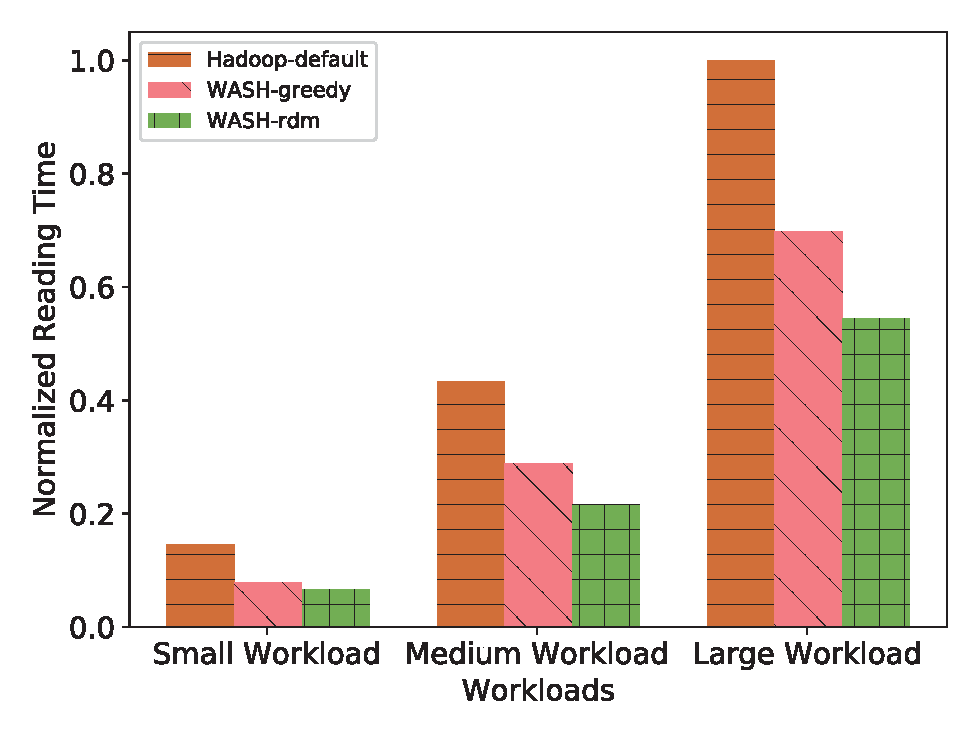
\includegraphics[height=1.6in]{figcomplete1_6.eps}}\quad\quad %quad 表示图像的间距
	\subfigure[Results under different Heterogeneity cluster. ]{\label{Fig:completeHeter}\includegraphics[height=1.6in]{figcomplete2_6.eps}}\quad\quad
	\subfigure[Results under various setting on replicas number
	]{\label{Fig:completeRep}\includegraphics[height=1.6in]{figcomplete3_6.eps}}
	\vspace{-1ex}
	\caption{Comparison of WASH-rdm and other Algorithm on different workloads, different heterogeneity cluster and different replica number $C$. \ref{Fig:completeWorkload} denotes effect of different workloads on reading time. \ref{Fig:completeHeter} denotes the reading time of the three algorithm on different Heterogeneity cluster. \ref{Fig:completeRep} denotes the reading time of the three algorithm when $C$ is different. Y-axis denotes the reading time of all tasks which has been normalized.}
	\label{Fig:complete}
	%\vspace{-1ex}
\end{figure*}

%\begin{table}[htbp]
%	\caption{THE DIFFERENT TRACES USED FOR EXPERIMENT}
%	\begin{center}
%		\begin{tabular}{|c|c|c|c|}
%			\hline
%			 \diagbox{Traces}{Number of tasks} & 1-150 & 150-500 & $\ge$ 500\\
%			\hline
%			Small Workload & 96\% & 2\% & 2\%\\
%			\hline
%			Medium Workload & 50\% & 40\% & 10\%\\
%			\hline
%			Large Workload & 40\% & 10\% & 50\%\\
%			\hline
%		\end{tabular}
%		\label{tab:workload}
%		\vspace{-0.4cm}
%	\end{center}
%\end{table}

\textbf{Settings:}
In traditional distributed file systems, e.g., HDFS\cite{b19}, data is distributed uniformly on disk. Therefore, in this experimental environment, we uniformly deploy 200000 data blocks each with three data replicas among 500 disks, whose unified size $\tau$ is 128MB. 500 disks are set up by default. The reading time of the disk for one piece of data, i.e., $T_i$, is a range from 10ms to 500ms, uniformly. 



\subsection{Simulation Results}

\textbf{Characteristic of task reading time.} Fig.~\ref{Fig:instance} shows the results under various workloads with 50 disks. X-axis represents the different disk ID. Y-axis represents the reading time of each disk by adopting the scheduling of the three algorithms. The lower peak curve has, the better performance the tasks have. The black dotted line represents the scheduling result of WASH-greedy, and the green line represents the scheduling result of Algorithm WASH-rdm. Overall, we can see that our proposed WASH-rdm performs much better than Hadoop-default. As shown in Fig.~\ref{Fig:instance1}, i.e., the small workload, the result of Hadoop-default has large fluctuations. This is a result of that scheduling of hadoop-default is not aware of the types and workloads of the disks when selecting a source device for a task. Even if the number of tasks that read data on disks are uniformly, the low-performances disks might have a relatively heavy use. As shown in Fig.~\ref{Fig:instance1}, disks with low-performance will have high peaks. 

Due to the completion of a job depending on the straggler task, the tasks reading data from the disks with poor performance could be the bottleneck of data analytical tasks. For example, in Hadoop-default, tasks reading data from disk-6, are the bottleneck of data analytics in the Fig.~\ref{Fig:instance1} which is 756. WASH-greedy and WASH-rdm could keep the reading time of disks roughly at a lower load, less than 450. The reason is that WASH-greedy can select the disk to read for the task according to performance of the disks where the maximum reading time of disks is 405.0 in disk-32. While WASH-rdm selects the source devices chooses source devices based on delicate calculated probabilities with peak 243.6 in disk-17. 
Compared with the Hadoop-default and WASH-greedy, our proposed WASH-rdm reduces reading time for tasks by up 67\% and 40\%, respectively.   

As the the number of tasks increasing, the reading time of each disk in data center also increases. Such as in Fig.~\ref{Fig:instance2}, when the number of tasks is about 2000, in Hadoop-default and WASH-greedy the maximum reading time among the disks is 2244 in disk-9 and 1495.0 in disk-22, respectively. While the maximum reading time of our proposed WASH-rdm is 1116 in disk-45, which speed up data analytics by up 51\% and 23\%, respectively. 
Furthermore, as shown in Fig.~\ref{Fig:instance3}, i.e., Large Workload,  When the number of tasks becomes larger, in the large Workloads of Fig.~\ref{Fig:instance3}, our proposed WASH-rdm could reduces reading time for tasks by up 57\% and 35\% over Hadoop-default and WASH-greedy, respectively. 


 %5546, 3650 and 2346

\textbf{Scalability of WASH.} Next, we focus on the impact of different factors, i.e., workloads, degree of heterogeneity and the number of data replicas, on the reading time of tasks upon the default configuration. In Fig.~\ref{Fig:completeWorkload}, the horizontal X-axis represents different workloads, and the Y-axis represents the maximum reading time among disks in the cluster, which has been normalized. In the previous part, the reading time of each disk show increasing trend with the workloads gets larger. 
Fig.~\ref{Fig:completeWorkload} shows the difference among the three workloads. The performance of our proposed HTS-rdm can always be improved by 55\% on average, over Hadoop-default. Next, we observed the effect of degree of heterogeneity on the load. We divide the heterogeneity of the cluster into two kinds. One is that the $T_i$ of disks is evenly distributed between 10ms and 100ms, named Low Heterogeneous Cluster. Another is High Heterogeneous Cluster, where the $T_i$ of disks are evenly distributed between 10ms and 500ms. Other conditions are configured by default. From Fig.~\ref{Fig:completeHeter}, when the degree of heterogeneity gets larger, the overall load shows an increasing trend. This is because the large the degree of heterogeneity, the greater the performance difference between disks. This leads to hard balancing of disk loads. Through \ref{Fig:completeHeter}, we find that our algorithm can also improve the performance of 40-50\% in clusters with high heterogeneity. Finally, we analyze the impact of the amount of data replicas on disk load. We set the number of data replicas as 2, 3 and 5. Observe that the higher the number of replicas, the lower the disk load. Reason for it is that with the number of data replicas increasing, the probability of data being deployed on high performance disks increases. Selecting data on high-performance disks at this time will greatly accelerate the completion of tasks. When $C$ = 5, our algorithm can achieve 65\% performance improvement.
 
 All in all,  the performance of the two algorithms proposed by us has reached an average of 55\% improvement over baseline algorithm on average under different conditions.



\section{CONCLUSION}\label{CONCLUSION}
In this paper, in order to avoid the unbalanced use on disks, as well as speed up the reading time of data analytical tasks, the types of heterogeneous storage devices and the workloads on storage devices should be both taken into consideration. Therefore, we formulate the workload-aware scheduling problem for heterogeneous storage devices, showing its NP-hardness and design a randomized algorithm which can be proved concentrated on its optimum with high probability through our theoretical analysis. The results of our simulations show that our proposed WASH-rdm speeds up data analytics up to 55\% over the baseline algorithms.
%\section*{Acknowledgment}
%None
\begin{comment} ... 
\section*{APPENDIX}

\textbf{\normalsize{The Proof of Theorem 1}}
\vspace{1ex}

The decision version of our WASH problem asks whether there exits a series of variables satisfying all the constrains (there is no objective function). Such problem can be reduced from 3-SAT problem which is defined as follows: Given a set of variables $B = \{b_1, b_2, ..., b_n\}$, each of them only can be taken in $\{True, False\}$. A literal $l$ consists of $b_i$ or $\overline b_i$. There are $m$ different clauses $C_j$, one of which is a disjunction of three literals \cite{b44}. The 3-SAT problem asks whether or not there exits a series of $b_i$ satisfying the total clauses which is one of Karp's 21 NP-complete problems \cite{b9}.

Taking the special case of  WASH problem, the parameters are set as follows:
\begin{itemize}
	\item $\mathcal{D}$ = \{1, 2, ..., 3\};
	$\mathcal{M}$ = \{1, 2, ..., n\}; 
	\item $C$ = 3.
\end{itemize}

Each variable $b_i$ has corresponding variable $I_l$.
For each clause like $b_1\wedge  b_2 \wedge b_3$, we have $I_1 + I_2 + I_3 = 1$. On one hand, if there exits a series of $b_i \in \{True, False\}$ satisfying the clauses, the constrains of WASH could be satisfied. On the other hand,  if there exits a series of $I_i \in \{1, 0\}$ satisfying the our constrains, the clauses of 3-SAT could be satisfied. \hfill \qedsymbol


The decision version of WASH problem is formulated as: Whether the optimum of WASH problem is less than $K$ or not.


The canonical form \cite{b11} of ILP is described below.

For $m\times n$ matrix \textbf{A}
\begin{align}
Min:&\;\;\;\;\;\textbf{c}^T\textbf{x}\;\;\;\;\;\;[\rm{ILP}]\label{ILP}\\
s.t. 
&\;\;\;\;\;\textbf{A}\textbf{x}\geq \textbf{b},\nonumber\\
&\;\;\;\;\;\textbf{x} \geq0\;and\;\textbf{x} \in \mathbb{Z}^n.\nonumber
\end{align}
Taking the special case of WASH problem, the parameters are set as follows:
\begin{itemize}
	\item $\mathcal{D}$ = \{$0$, $1$, $2$\};$T_0$ = 1, $T_1$ = 1, $T_2$=1; $\mathcal{M}$ = \{$0$, $1$, ..., $n-1$\}; $C$ = 3
	\item $T$ = \{$0$, $1$, ..., $n-1$\}
\end{itemize}

It means that there are 3 disks, $0$, $1$, $2$, in the data center, each disk with a $T_i$ of 1. A total of n data, and each data has three replicas which deployed in the three disks, respectively. When the query job arrives, the job is divided into n tasks, \{$t0$, $1$, ..., $n$\} to read n data, \{$0$, $1$, ..., $n$\}, respectively.

For this particular case, the problem description can be modified to:
\begin{align}
Min:&\;\;\;\;\;\max\{\sum_{j}I_0^j, \sum_{j}I_1^j, \sum_{j}I_2^j\}\;\;\;\;\;[\rm{WASH-sp}]\nonumber\\
s.t. 
&\;\;\;\;\;I_0^j + I_1^j +I_2^j= 1,\;\;\forall j,\nonumber\\
&\;\;\;\;\;I_0^j, I_1^j, I_2^j\in\{0,1\},\;\;\forall j \in[0,n).\nonumber
\end{align}

Let  $x$ = $\sum_{j}I_0^j$, $y$ = $\sum_{j}I_1^j$, $z$ = $\sum_{j}I_2^j$, and the problem description can be modified to:
\begin{align}
Min:&\;\;\;\;\;\max\{x,y,z\}\;\;\;\;\;\;[\rm{WASH-sp}]\\
s.t. 
&\;\;\;\;\;x + y + z = n,\;\label{enlarge-cons}\\
&\;\;\;\;\;0 \leq x, y, z \leq n  \;\;x, y, z\in\mathbb{Z}.\nonumber
%&\;\;\;\;\;0 \leq y \leq n, y\in\mathbb{Z}\nonumber\\
%&\;\;\;\;\;0 \leq z \leq n, z\in\mathbb{Z}\nonumber
\end{align}
In the minimization problem, x + y + z = n can be modified to x + y + z = n and let $R$ denotes $\max\{x,y,z\}$. 

Finally, WASH-sp problem is converted to:
\begin{align}
Min:&\;\;\;\;\;0*x+0*y+0*z+R\;\;\;\;\;\;\;[\rm{WASH-ILP}]\label{WASH-ILP}\nonumber\\
s.t. 
&\;\;\;\;\;x + y + z \geq n,\;\nonumber\\
&\;\;\;\;\;-x + R \geq 0, \nonumber\\
&\;\;\;\;\;-y + R \geq 0, \nonumber\\
&\;\;\;\;\;-z + R \geq 0, \nonumber\\
&\;\;\;\;\;0 \leq x, y, z \leq n  \;\;x, y, z\in\mathbb{Z},\nonumber\\
%&\;\;\;\;\;0 \leq x \leq n, x\in\mathbb{Z}\nonumber\\
%&\;\;\;\;\;0 \leq y \leq n, y\in\mathbb{Z}\nonumber\\
%&\;\;\;\;\;0 \leq z \leq n, z\in\mathbb{Z}\nonumber\\
&\;\;\;\;\;R \geq 0, R\in\mathbb{Z}.\nonumber
\end{align}
%(\ref{WASH-ILP})
Obviously, WASH-ILP  is an instance of ILP in (\ref{ILP}). The decision version of 0-1 ILP (A variation in which only the restrictions must be satisfied, without optimization) is one of Karp's 21 NP-complete problems \cite{b9}, so ILP is NP-hard. Further, the WASH-ILP problem is NP-hard.

On the one hand, when the optimal solution of WASH-ILP problem is obtained, the corresponding {x, y, z} can be converted into variable {$I_i^j$} thin polynomial time by setting the value in \{$I_0^0$, $I_0^1$, ...,$I_0^{x-1}$, $I_1^{x}$, $I_1^{x+1}$, ..., $I_1^{x+y-1}$, $I_2^{x+y}$, $I_1^{x+y+1}$, ..., $I_2^{x+y+z-1}$\} to be 1, which will make the corresponding WASH-sp problem obtain the optimal solution. On the other hand, when the variable \{$I_i^j$\} make the WASH-sp problem obtain the optimal solution, the WASH-ILP also obtains the optimal solution by setting $x$ = $\sum_{j}I_0^j$, $y$ = $\sum_{j}I_1^j$, $z$ = $\sum_{j}I_2^j$. It can be seen from the above that any solution can be polynomially transformed between the WASH-sp and WASH-ILP. Therefore, WASH-sp is NP-hard. 

As a result of that WASH-sp is a special case in WASH, WASH problem is NP-hard.\hfill $\qedsymbol$
\end{comment}


\begin{thebibliography}{00}
\bibitem{b1} Ahmad F, Chakradhar S T, Raghunathan A, et al. Tarazu: optimizing mapreduce on heterogeneous clusters[C]//ACM SIGARCH Computer Architecture News. ACM, 2012, 40(1): 61-74.
\bibitem{b2} Zaharia M, Borthakur D, Sen Sarma J, et al. Delay scheduling: a simple technique for achieving locality and fairness in cluster scheduling[C]//Proceedings of the 5th European conference on Computer systems. ACM, 2010: 265-278.
\bibitem{b3} Ananthanarayanan G, Agarwal S, Kandula S, et al. Scarlett: coping with skewed content popularity in mapreduce clusters[C]//Proceedings of the sixth conference on Computer systems. ACM, 2011: 287-300.
\bibitem{b4} Abad C L, Lu Y, Campbell R H. DARE: Adaptive data replication for efficient cluster scheduling[C]//2011 IEEE international conference on cluster computing. IEEE, 2011: 159-168.
\bibitem{b5} Jalaparti V, Bodik P, Menache I, et al. Network-aware scheduling for data-parallel jobs: Plan when you can[C]//ACM SIGCOMM Computer Communication Review. ACM, 2015, 45(4): 407-420.
\bibitem{b6} Xu L, Butt A R, Lim S H, et al. A heterogeneity-aware task scheduler for spark[C]//2018 IEEE International Conference on Cluster Computing (CLUSTER). IEEE, 2018: 245-256.
\bibitem{b7} Pan F, Xiong J, Shen Y, et al. H-Scheduler: Storage-Aware Task Scheduling for Heterogeneous-Storage Spark Clusters[C]//2018 IEEE 24th International Conference on Parallel and Distributed Systems (ICPADS). IEEE, 2018: 1-9.
\bibitem{b8} Wang B, Jiang J, Yang G. Actcap: Accelerating mapreduce on heterogeneous clusters with capability-aware data placement[C]//2015 IEEE Conference on Computer Communications (INFOCOM). IEEE, 2015: 1328-1336.
\bibitem{b9} Karp R M. Reducibility among combinatorial problems[M]//Complexity of computer computations. Springer, Boston, MA, 1972: 85-103.
\bibitem{b10} Hromkovič J. Algorithmics for hard problems: introduction to combinatorial optimization, randomization, approximation, and heuristics[M]. Springer Science \& Business Media, 2013.
\bibitem{b11} 2018. Integer programming.     https://en.wikipedia.org/wiki/Integer\_progr- amming.
\bibitem{b12} Grimmett G, Grimmett G R, Stirzaker D. Probability and random processes[M]. Oxford university press, 2001.
\bibitem{b13} 2019. Martingale (probability theory). https://en.wikipedia.org/wiki/Martingale\_(probability\_theory)

\bibitem{b14} Wang B, Jiang J, Yang G. Actcap: Accelerating mapreduce on heterogeneous clusters with capability-aware data placement[C]//2015 IEEE Conference on Computer Communications (INFOCOM). IEEE, 2015: 1328-1336.
\bibitem{b15} Apache Spark. https://spark.apache.org, 2019.
\bibitem{b16}Seagate. https://www.seagate.com/cn/zh/.
\bibitem{b17}Samsung. https://www.samsung.com/semiconductor/cn/, 2019.
\bibitem{b18}Guo Z, Fox G, Zhou M. Investigation of data locality in mapreduce[C]//Proceedings of the 2012 12th IEEE/ACM International Symposium on Cluster, Cloud and Grid Computing (ccgrid 2012). IEEE Computer Society, 2012: 419-426. 
\bibitem{b19} Hdfs. https://hadoop.apache.org/hdfs, 2019.
\bibitem{b20} 2012. Google Cluster Trace. https://code.google.com/p/googleclusterdata/.

\bibitem{b25} F. Ahmad, S. Chakradhar A. Raghunathan and T. N. Vijaykumar. Tarazu: optimizing mapreduce on heterogeneous clusters. In ACM ASPLOS 2012.
\bibitem{b26} R. Gandhi, D. Xie, Y. Charlie. PIKACHU: How to Rebalance Load in Optimizing MapReduce On Heterogeneous Clusters. In USENIX ATC 2013.
\bibitem{b27}Malik M, Neshatpour K, Rafatirad S, et al. Hadoop workloads characterization for performance and energy efficiency optimizations on microservers[J]. IEEE Transactions on Multi-Scale Computing Systems, 2017, 4(3): 355-368.
\bibitem{b28}Gupta P K. Accelerating datacenter workloads[C]//26th International Conference on Field Programmable Logic and Applications (FPL). 2016.

\bibitem{b29}Kong J. Datacenter storage system: U.S. Patent Application 13/694,001[P]. 2014-4-24.
\bibitem{b30}Delimitrou C, Sankar S, Vaid K, et al. Decoupling datacenter studies from access to large-scale applications: A modeling approach for storage workloads[C]//2011 IEEE International Symposium on Workload Characterization (IISWC). IEEE, 2011: 51-60.
\bibitem{b31}Guo Y, Gong Y, Fang Y, et al. Energy and network aware workload management for sustainable data centers with thermal storage[J]. IEEE Transactions on Parallel and Distributed Systems, 2013, 25(8): 2030-2042.
\bibitem{b32} HDD. https://en.wikipedia.org/wiki/Hard\_disk\_drive
\bibitem{b33} SSD. https://en.wikipedia.org/wiki/Solid\-state\_drive
\bibitem{b34} Oceanbase. http://oceanbase.org.cn/?p=151. 2016-3-25.
\bibitem{b35}Stone J E, Gohara D, Shi G. OpenCL: A parallel programming standard for heterogeneous computing systems[J]. Computing in science \& engineering, 2010, 12(3): 66.
\bibitem{b36}Xie J, Yin S, Ruan X, et al. Improving mapreduce performance through data placement in heterogeneous hadoop clusters[C]//2010 IEEE International Symposium on Parallel \& Distributed Processing, Workshops and Phd Forum (IPDPSW). IEEE, 2010: 1-9.

\bibitem{b37}Stuedi P, Trivedi A, Pfefferle J, et al. Crail: A High-Performance I/O Architecture for Distributed Data Processing[J]. IEEE Data Eng. Bull., 2017, 40(1): 38-49.

\bibitem{b38}Zumberge J F, Urban M P, Liu R, et al. International GPS Service for Geodynamics[J]. 1996.

\bibitem{b39}Kern M, Culhane S, Hoffman D. Systems, Methods and Media for Distributing Peer-to-Peer Communications: U.S. Patent Application 14/035,945[P]. 2014-1-23.


\bibitem{b40}Apache Storm. https://storm.apache.org.

\bibitem{b41}Dean J, Ghemawat S. MapReduce: simplified data processing on large clusters[J]. Communications of the ACM, 2008, 51(1): 107-113.

\bibitem{b42}Davidson A, Or A. Optimizing shuffle performance in spark[J]. University of California, Berkeley-Department of Electrical Engineering and Computer Sciences, Tech. Rep, 2013.

\bibitem{b43}Mitzenmacher M. The power of two choices in randomized load balancing[J]. IEEE Transactions on Parallel and Distributed Systems, 2001, 12(10): 1094-1104.
\bibitem{b44}Lynce I, Ouaknine J. Sudoku as a SAT Problem[C]//ISAIM. 2006.
\end{thebibliography}
\end{document}

